% !TEX root=./report.tex

\subsection{Static Calibration}
\label{sec:static_calibration_approach}

ITS are inherently dependent on the calibration of the different sensors. 
The system has to know the poses of the different sensors relative to some reference coordinate system to accurately measure the position of vehicles within the single sensor ranges and at the overlapping boundaries.

We propose a calibration procedure based on a Bundle Adjustment (BA) problem formulation.
We map visual landmarks in the video feed to their partially known world positions from high definition road maps (HD maps).
We recover the pose by jointly optimizing for the camera intrinsic and extrinsic parameters as well as the real world positions of the landmarks. 

%%%%%%%%%%%%%%%%%%%%%%%%%%%%%%%%%%%%%%%%%%%%%%%%%%%%%%%%%%%%%%%%%%%%%%%%%%%%%%%%%%%%%%%%%%%%%%%%%%%%%%%%%%%%%%%%%%%%%%%%%%%%%%%%%%%%%%%%%%%%%%%%%%%%%%%%%%%%%%%%%
%%%%%%%%%%%%%%%%%%%%%%%%%%%%%%%%%%%%%%%%%%%%%%%%%%%%%%%%%%%%%%%%%%%%%%%%%%%%%%%%%%%%%%%%%%%%%%%%%%%%%%%%%%%%%%%%%%%%%%%%%%%%%%%%%%%%%%%%%%%%%%%%%%%%%%%%%%%%%%%%%
%%%%%%%%%%%%%%%%%%%%%%%%%%%%%%%%%%%%%%%%%%%%%%%%%%%%%%%%%%%%%%%%%%%%%%%%%%%%%%%%%%%%%%%%%%%%%%%%%%%%%%%%%%%%%%%%%%%%%%%%%%%%%%%%%%%%%%%%%%%%%%%%%%%%%%%%%%%%%%%%%

\paragraph{Retrieve Objects from High Definition Maps}

In our project we use HD maps in the \OD{} standard format.
In this work we focus on the permanent delineator (PD) objects that are easily visible in the video feeds.

We extract the world position of the PDs using the mathematical operations defined in the \OD{} standard.
This gives us the base origin point $o~=~(x, y, z)^T$ of the PDs in the Universal Transverse Mercator (UTM) projection \cite{langley1998utm,proj}. 
The point $o$ is the real world position of the lower end of the PD where it touches the ground or another object.
Additionally, we retrieve a directional heading axis $d~=~(x, y, z)^T$ and the height $h$ of the PD.

\paragraph{1D Approximation of Objects}

In the original BA setting the optimization is done jointly over multiple cameras and observations, and the arising stereo vision problem is solved jointly for the 3D positions of the objects and the camera parameters.
For this system of equations to be solvable it requires multiple cameras from different viewing angles and large overlapping fields of view between the cameras.

In our project we have neither of the requirements and thus calibrate each camera separately to the HD map.
We relax the BA problem by the 1D line approximation of the PDs
\begin{equation}
S = \{o + \lambda * d: \quad \lambda \in [0, h]\}
\end{equation}
where $S$ is the set of points along its central axis between the base at $\lambda = 0$ and its top at $\lambda = h$.
This approximation allows for a joint optimization of their world positions and the camera intrinsic and extrinsic parameters.

\Cref{sec:static_calibration_number_points} derives a minimal number of points for the resulting system of equations to be solvable.

% The assumptions we made are: 
% \begin{itemize}
  % \item Objects are symmetric around their directional heading axis.
  % \item Projected pixels of the objects are also symmetric around the projected directional axis.
% \end{itemize}


%%%%%%%%%%%%%%%%%%%%%%%%%%%%%%%%%%%%%%%%%%%%%%%%%%%%%%%%%%%%%%%%%%%%%%%%%%%%%%%%%%%%%%%%%%%%%%%%%%%%%%%%%%%%%%%%%%%%%%%%%%%%%%%%%%%%%%%%%%%%%%%%%%%%%%%%%%%%%%%%%
%%%%%%%%%%%%%%%%%%%%%%%%%%%%%%%%%%%%%%%%%%%%%%%%%%%%%%%%%%%%%%%%%%%%%%%%%%%%%%%%%%%%%%%%%%%%%%%%%%%%%%%%%%%%%%%%%%%%%%%%%%%%%%%%%%%%%%%%%%%%%%%%%%%%%%%%%%%%%%%%%
%%%%%%%%%%%%%%%%%%%%%%%%%%%%%%%%%%%%%%%%%%%%%%%%%%%%%%%%%%%%%%%%%%%%%%%%%%%%%%%%%%%%%%%%%%%%%%%%%%%%%%%%%%%%%%%%%%%%%%%%%%%%%%%%%%%%%%%%%%%%%%%%%%%%%%%%%%%%%%%%%

\paragraph{Mapping Objects to Pixels}
\begin{figure}[t]
  \centering
  \begin{tabular}{c}
     \includegraphics[width=0.95\linewidth]{images/hd_map_mapping.png}
    \end{tabular}
    \caption{
       Left: The current camera frame. 
       Right: A part of the HD map.
       Light blue lines: An exemplary mapping $s_c \mapsto p_c$ from objects (right) to their corresponding pixels (left).
       }
  \label{fig:static_calibration_mapping}
  \end{figure}

We solve the BA problem by minimizing the reprojection-error over the PDs.
We thus require a set $C$ of correspondences that map world points $s_c$ of the PDs to their respective pixel $p_c$. 
\Cref{fig:static_calibration_mapping} displays an exemplary mapping from a HD map to the video feed.

This mapping is currently done by human interaction and not fully automated. 
We implemented an annotation tool to mark pixels that outputs a list of pixels that can easily be mapped to the list of objects.

%%%%%%%%%%%%%%%%%%%%%%%%%%%%%%%%%%%%%%%%%%%%%%%%%%%%%%%%%%%%%%%%%%%%%%%%%%%%%%%%%%%%%%%%%%%%%%%%%%%%%%%%%%%%%%%%%%%%%%%%%%%%%%%%%%%%%%%%%%%%%%%%%%%%%%%%%%%%%%%%%
%%%%%%%%%%%%%%%%%%%%%%%%%%%%%%%%%%%%%%%%%%%%%%%%%%%%%%%%%%%%%%%%%%%%%%%%%%%%%%%%%%%%%%%%%%%%%%%%%%%%%%%%%%%%%%%%%%%%%%%%%%%%%%%%%%%%%%%%%%%%%%%%%%%%%%%%%%%%%%%%%
%%%%%%%%%%%%%%%%%%%%%%%%%%%%%%%%%%%%%%%%%%%%%%%%%%%%%%%%%%%%%%%%%%%%%%%%%%%%%%%%%%%%%%%%%%%%%%%%%%%%%%%%%%%%%%%%%%%%%%%%%%%%%%%%%%%%%%%%%%%%%%%%%%%%%%%%%%%%%%%%%

\paragraph{Calibration Procedure}
\begin{figure}[t]
  \centering
  \begin{tabular}{c}
    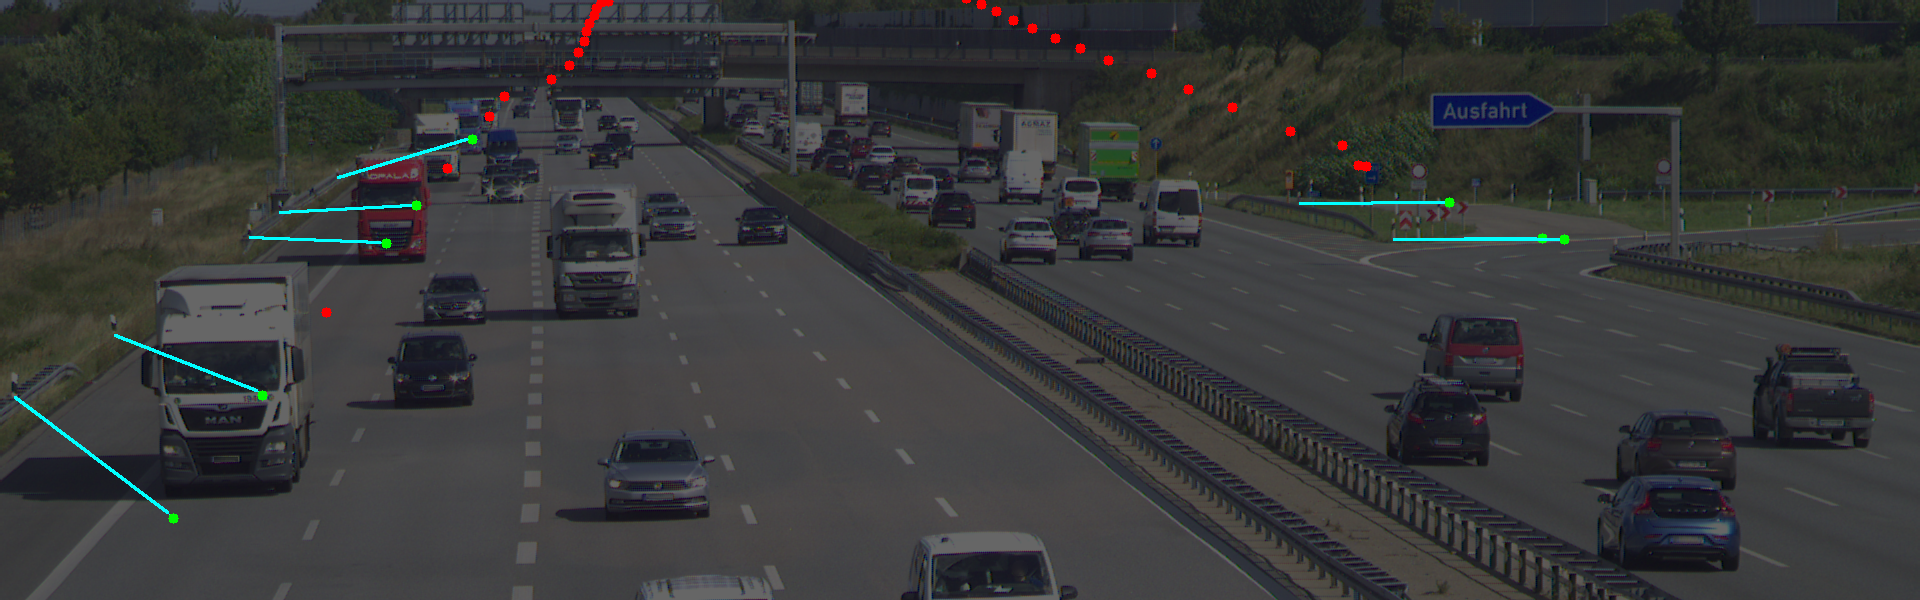
\includegraphics[width=0.95\linewidth]{images/calibration/background_uncalibrated_with_mapping.png}    \\
    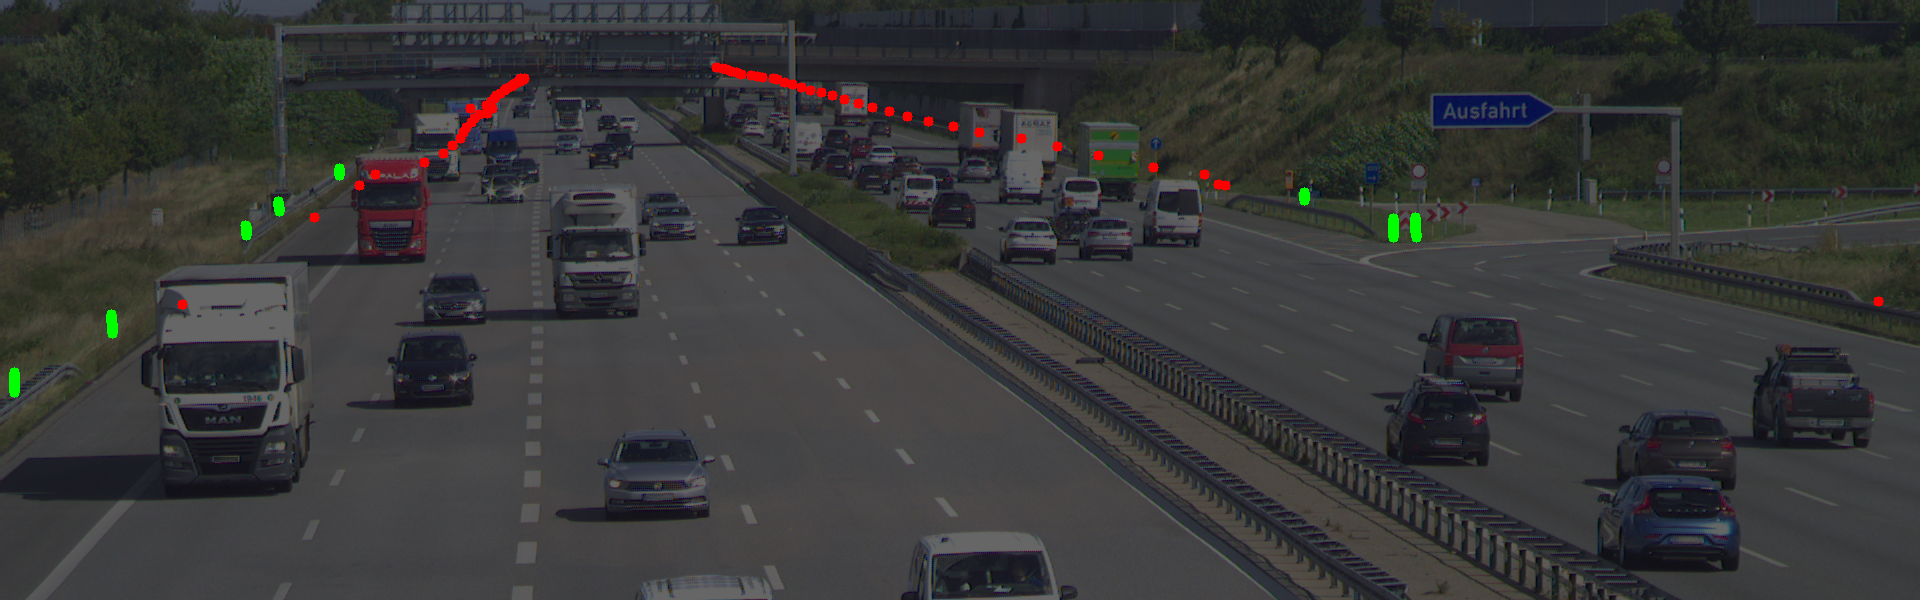
\includegraphics[width=0.95\linewidth]{images/calibration/background_calibrated.png}    
  \end{tabular}
  \caption{
    Top: Points of PDs mapped to pixel locations (green) and points without known corresponding pixels (red) rendered by a poorly calibrated camera model.
    The mapping from the projected points to their expected pixels is drawn in light blue.
    Bottom: The same points after the calibration procedure.
    The rendered positions of the mapped points align with their respective pixels.
    The drawn mapping disappears as the distances approach $0$.
   }
  \label{fig:static_calibration_calibration}
\end{figure}
  
We model our cameras using the pinhole camera model. 
The projection from points $s_c~=~o_c~+~\lambda_c~*~h_c$ of the PDs world positions to pixels $p_c$ is formulated as

\begin{equation}
  \label{eq:static_calibration_reprojection}
  p_c = \pi \left( R * T * (o_c + \lambda_c * h_c) \right)
\end{equation}

where $R$ is the cameras world rotation in Euler angles, $T$ is the cameras world translation and $\pi$ is the pinhole projection to image space based on the camera intrinsic parameters.
The pinhole projection $\pi$ is formulated as

\begin{equation}
  \label{eq:static_calibration_intrinsic_parameters}
  z * \pi(x) =   
  \begin{pmatrix}
    f_x,& 0,& c_x,& 0\\
    0,& f_y,& c_y,& 0\\
    0,& s,& 1 ,& 0
  \end{pmatrix} * x 
\end{equation}

where $x$ is an 3D input vector in homogeneous coordinates, $f_x, f_y$ are the focal lengths in pixels, $c_x, c_y$ is the principle point, $s$ is the skew parameter and $z$ is the homogeneous component used in the perspective division. 

The optimal values for $\pi,R,T$ are found if for all correspondences the distance between the expected pixel $\hat{p}_c$ and the projected pixel $p_c$ is minimal and it holds for all $c$
\begin{equation}
  0 = \hat{p}_c - \pi \left( R * T * (o_c + \lambda_c * h_c)\right) = \hat{p}_c - p_c
\end{equation}

This places constraints on the values $\pi,R,T$ can take and enables us to recover the camera pose, the intrinsic parameters and the 1D approximate positions relative to the $\lambda$s only from the correspondences.\\
\Cref{fig:static_calibration_calibration} displays rendering the PDs before and after calibration.

%%%%%%%%%%%%%%%%%%%%%%%%%%%%%%%%%%%%%%%%%%%%%%%%%%%%%%%%%%%%%%%%%%%%%%%%%%%%%%%%%%%%%%%%%%%%%%%%%%%%%%%%%%%%%%%%%%%%%%%%%%%%%%%%%%%%%%%%%%%%%%%%%%%%%%%%%%%%%%%%%
%%%%%%%%%%%%%%%%%%%%%%%%%%%%%%%%%%%%%%%%%%%%%%%%%%%%%%%%%%%%%%%%%%%%%%%%%%%%%%%%%%%%%%%%%%%%%%%%%%%%%%%%%%%%%%%%%%%%%%%%%%%%%%%%%%%%%%%%%%%%%%%%%%%%%%%%%%%%%%%%%
%%%%%%%%%%%%%%%%%%%%%%%%%%%%%%%%%%%%%%%%%%%%%%%%%%%%%%%%%%%%%%%%%%%%%%%%%%%%%%%%%%%%%%%%%%%%%%%%%%%%%%%%%%%%%%%%%%%%%%%%%%%%%%%%%%%%%%%%%%%%%%%%%%%%%%%%%%%%%%%%%

\paragraph{Reprojection-Error Formulation}
\label{sec:static_calibration_rerpojection_error}
We solve the BA problem by minimizing a modified version of the least-squares reprojection-error $E$ formulated as

\begin{equation}
  \begin{split}
  E(P, S, \pi, T, R, W ) =& 
  \sum_{c \in C} 
  \rho(\left\lVert 
    w_c * [ \hat{p}_c - p_c ]
  \right\rVert^2_2) \\ 
  +& 
  \sum_{c \in C} 
  \alpha * 
  \rho(\left\lVert 
  (1 - w_c)
  \right\rVert^2_2) \\ 
  +& 
  \sum_{c \in C} 
  \beta * 
  \rho(\left\lVert 
  \Delta(\lambda_c, 0, h_c)
  \right\rVert^2_2) \\ 
  +& 
  \sum_{\pi_i \in \pi} 
  \gamma *
  \rho(\left\lVert 
  \Delta (\pi_i, \pi_i * 0.9, \pi_i * 1.1)
  \right\rVert^2_2) \\
  +&
  \delta * 
  \rho(\left\lVert 
  \Delta (R_x, 60, 110)
  \right\rVert^2_2) \\
  +&
  \delta * 
  \rho(\left\lVert 
  \Delta (R_y, -10, 10)
  \right\rVert^2_2 
\end{split}
\label{eq:static_calibration_rerpojection_error}
\end{equation}

where $P$ is the set of mapped pixels $\hat{p}_c$ in the image and $S$ is the set of mapped corresponding points $s_c$ from the PDs.  
The additional weights $w_c \in W$ are associated to the correspondences to downweight outliers and are enforced to stay near $1$.
We use a robust loss function $\rho$ to further decrease the influence of outliers.

We guide the algorithm to feasible solutions by penalizing $\lambda_c$ values that are negative or exceed the PDs height $h_c$ using the distance 
\begin{equation}
    \Delta (x, l, u) =
    \begin{cases}
      x - u,& \text{if } x > u\\
      x - l,& \text{if } x < l\\
      0,    & \text{else}
    \end{cases} 
\end{equation}
from the interval $[l, u]$.

We rely on a rough initialization for the values $\pi_i \in \pi$ and allow the optimizer to adjust the values within a $\pm 0.1$ interval around the initialization. 

Finally, we constrain the $X$ axis rotation $R_x$ (Pitch) to be within the interval $[60, 110]$ degree and the $Y$ axis rotation $R_y$ (Roll) to be within the interval $[-10, 10]$ degree, meaning that the camera has to be roughly in level and face horizontally.

The factors $\alpha, \beta, \gamma, \delta$ are used to explicitly scale the remaining losses of the terms, thus giving them different influence on the optimizer. 
We saw empirically that good values for the factors are $\alpha = 1*10^{100}, \beta = 2, \gamma = 10, \delta = 50$.

\paragraph{Initialization}
In contrast to most BA problems our approach drops the need for good initialization. 
The regularization of the $\lambda$ values gives the optimizer enough flexibility to optimize over the infinite space of possible values, but enforces the values of the $\lambda$ to lie within the interval of $\lambda \in [0, h]$.

The optimizer calculates its own initial guess
\begin{equation}
  T_0 = T(\bar{s}_x, \bar{s}_y, \bar{s}_z + \bar{d}) 
\end{equation}
for the camera translation based on the mean 
\begin{equation}
  \bar{s} = \frac{1}{\left\lvert C \right\rvert } \sum_{c \in C} o_c
\end{equation}
of the base origin points $o_c$ of the PDs and some distance $\bar{d}$ from the mean.

The optimizer initializes the rotation  
\begin{equation}
  R_0 = R(x, y, z)
\end{equation}
based on $x, y, z$ Euler angle values drawn from the uniform distribution $U(-35, 35)$, where $R(0,0,0)$ is the camera facing in negative $Z$ direction onto the mean $\bar{s}$.
This initialization ensures that all points lie in front of the camera and can be projected onto the image plane.

It is sufficient to initialize $\lambda_c = 0$ for all correspondences.